\documentclass[10pt,a4paper,twocolumn]{article}
\usepackage[T1]{fontenc}
\usepackage{mathptmx}
\usepackage{courier}
\usepackage[top=2cm,bottom=2.2cm,left=1.7cm,right=1.7cm,columnsep=0.6cm]{geometry}
\usepackage{microtype,amsmath,tabularx,enumitem,xcolor,listings,tikz,caption,fancyhdr,titlesec,array}
\usepackage{pgfplots}\pgfplotsset{compat=1.17}
\usepackage[hidelinks]{hyperref}
\usetikzlibrary{positioning,fit,arrows.meta}

\setlist{itemsep=1pt,topsep=2pt,leftmargin=*}
\captionsetup{font=footnotesize,labelfont=bf,labelsep=period}
\captionsetup[table]{position=top,skip=3pt}
\titleformat{\section}{\normalsize\bfseries\scshape}{\thesection.}{0.5em}{}
\titleformat{\subsection}{\normalsize\bfseries\itshape}{\thesubsection}{0.5em}{}
\titlespacing*{\section}{0pt}{10pt}{4pt}
\titlespacing*{\subsection}{0pt}{7pt}{3pt}
\renewcommand{\arraystretch}{1.2}
\setlength{\tabcolsep}{4pt}
\newcolumntype{L}{>{\raggedright\arraybackslash}X}
\newcolumntype{C}{>{\centering\arraybackslash}X}

\pagestyle{fancy}\fancyhf{}
\fancyhead[C]{\footnotesize\itshape Counter-Based Performance Attribution on Heterogeneous Embedded Hardware}
\fancyfoot[C]{\footnotesize\thepage}
\renewcommand{\headrulewidth}{0.4pt}

\lstset{language=C,basicstyle=\ttfamily\scriptsize,frame=single,rulecolor=\color{black},
  framesep=3pt,xleftmargin=4pt,xrightmargin=4pt,columns=fullflexible,keepspaces=true,
  commentstyle=\itshape,keywordstyle=\bfseries,showstringspaces=false,aboveskip=5pt,belowskip=5pt,
  captionpos=b}
\renewcommand{\lstlistingname}{Listing}
\newcommand{\code}[1]{\texttt{\small #1}}

\begin{document}
\twocolumn[{%
\begin{center}
{\LARGE\bfseries A Counter-Based Harness for Profiling How\\[3pt] Heterogeneous Embedded Hardware Runs Any Program\par}
\vspace{10pt}
\begin{minipage}{0.86\textwidth}\small
\textbf{\textit{Abstract}---}A program's run time on an embedded board shows \emph{how long} it takes, but not \emph{why}. The same code can be limited by arithmetic on one board, by external memory on another, and by the scheduler sharing a core on a third, and a duration cannot separate these cases. We present a small, portable C harness that profiles how a board runs an arbitrary, unmodified program. A one-time \emph{hardware sweep} measures the board's own prices: its peak instruction throughput, the cost of waiting for a dependent arithmetic result, the latency of each memory tier, and the cost of a miss at each cache level. On Linux boards the harness launches the program, attaches hardware performance counters to every thread before its first instruction, and reads them when the thread exits, so neither the code nor its number of threads needs to be known. For each thread it reports what the code did (instruction mix, branches, misses per level) and where its time went, divided into five categories that are identical on every board---COMPUTE, MEMORY, STALLED, KERNEL and WAITING---with sub-categories (cache level, arithmetic wait, preempted or blocked) where the board's counters allow. It separates visible delays from memory latency hidden by out-of-order execution, labels each thread with its dominant cause, and states how much of the measured time it explains. One source file targets the Raspberry Pi~5, the Jetson Orin Nano, the ESP32-P4 and the GAP9, degrading gracefully where counters are missing. A validation program with no harness calls, whose threads each have a known behaviour, is described. A preliminary test on a laptop, in a Linux virtual machine without access to hardware counters, confirms that the harness finds every thread of an unmodified program, separates running, preempted and blocked time as expected, recovers the memory tiers from timing alone, and reports explicitly what it cannot measure.

\vspace{4pt}\noindent\textbf{\textit{Index Terms}---}hardware performance counters, performance attribution, memory hierarchy, out-of-order execution, scheduling, embedded systems, microcontrollers.
\end{minipage}
\end{center}
\vspace{12pt}}]
\thispagestyle{fancy}

\section{Introduction}

Embedded systems for perception and signal processing are deployed on very different hardware: Linux single-board computers with out-of-order cores, multi-level caches and DRAM; RISC-V microcontrollers with in-order cores, tightly-coupled memory and external PSRAM; and parallel ultra-low-power processors with software-managed memories. When one application moves between such boards, it does not slow down uniformly. A thread that is arithmetic-bound on a microcontroller may be memory-bound on a board with a small last-level cache, and a thread may look slow only because the scheduler gave its core to another.

A designer choosing or optimising a board therefore needs to know which resource limits each part of the program on each board. Existing tools address part of this need. Benchmarks and timing harnesses report durations without causes. Memory micro-benchmarks such as lmbench~\cite{lmbench} characterise the memory hierarchy, but not a program. Counter interfaces such as Linux \code{perf}~\cite{perfman} and PAPI~\cite{papi} expose raw counts and leave their interpretation open. Analytical methods such as the Roofline model~\cite{roofline} and Top-Down analysis~\cite{topdown} explain bottlenecks, but assume particular processor families or counter sets, or an analysis of the program's operations. In our review we found no tool that, for an arbitrary program, explains each thread's time in a vocabulary that stays the same on boards with and without caches, with and without an operating system, and that states how reliable that explanation is.

We designed a harness to fill that gap. Our contributions are:
\begin{enumerate}
  \item an \textbf{attribution model} that converts counted work into expected cycles using prices measured on the board, and divides each thread's time into five board-independent categories with board-dependent sub-categories;
  \item a \textbf{hardware sweep} that measures those prices without datasheet values or knowledge of the cache organisation;
  \item a \textbf{run mode} that profiles any unmodified Linux program, finding every thread automatically;
  \item a \textbf{delay breakdown} that separates time the core actually lost from memory latency hidden by out-of-order execution, and time preempted from time blocked;
  \item a \textbf{portable implementation} for Linux, ESP-IDF and PMSIS in which every counter is optional and validated;
  \item a \textbf{validation program} with no harness calls, whose threads each have a known behaviour.
\end{enumerate}

\section{Background}

\paragraph{Hardware performance counters.} Most processors contain a performance monitoring unit (PMU): a few registers that count hardware events such as cycles, retired instructions, loads, floating-point operations, branch mispredictions and cache refills. They observe a program without modifying it. Linux exposes them per thread through \code{perf\_event\_open}~\cite{perfman}; microcontroller SDKs expose a cycle counter and, on some chips, a few event counters~\cite{espidf,gapsdk}. A core has only a handful of counters (six programmable counters on the Cortex-A76 and A78AE), so when more events are requested, Linux time-multiplexes them and reports for how long each was active, from which the full count is estimated.

\paragraph{Memory hierarchy.} A load is served by the nearest memory that holds the data: a cache level or DRAM on a Linux board; TCM, internal SRAM, or PSRAM behind a cache on a microcontroller. Each tier has a characteristic latency, and an access that misses a tier pays the latency of the next.

\paragraph{In-order and out-of-order cores.} An in-order core, such as the RISC-V cores of the ESP32-P4 and GAP9, stops when a load misses and resumes when the data arrives, so the time lost is close to the number of misses multiplied by their latency. An out-of-order core, such as the Cortex-A78AE of the Jetson Orin Nano or the Cortex-A76 of the Raspberry Pi~5, continues to execute independent instructions while loads wait, and keeps several misses in flight. Much of the memory latency is then \emph{hidden}: it occurs, but overlaps useful work. These cores count the cycles in which no instruction could issue because the back end was waiting~\cite{topdown}, which measures the \emph{exposed} part directly. The same holds for arithmetic: a chain of dependent floating-point operations waits on each result, while independent operations overlap.

\paragraph{Running, preempted and blocked.} A thread's lifetime includes time it was not running. It may be \emph{preempted}, ready to run while the scheduler gives its core to another thread, or \emph{blocked}, sleeping or waiting for I/O or a lock. Linux records, per thread, the time spent running and the time spent ready but waiting (\code{schedstat}); the remainder of the lifetime is blocked. FreeRTOS records each task's running time when run-time statistics are enabled.

\section{Harness design}

\subsection{Goal and requirements}
The harness must (R1) work with any program, unchanged, without knowing how many threads it creates; (R2) work on any board, using whatever counters exist and producing a correct, if less detailed, report where some are missing; (R3) report, for every thread, what the code did and how its time divides among compute, memory (by level where possible), other stalls, the operating system and waiting; (R4) separate visible from hidden delays; (R5) use the same top-level categories on every board, so that boards can be compared; (R6) state how much of the measured time is explained; and (R7) be small enough to be read and verified line by line.

\subsection{Architecture}
Figure~\ref{fig:arch} shows the structure. The implementation, \code{pmu.c}, has two parts. \textbf{Part A}, the platform layer, is the only code that differs between boards: it opens and reads the counters (per thread where the board allows), provides the clocks, reports which threads or tasks used the core, and lists the board's memory regions. The compiler keeps exactly one platform section; an unknown platform stops compilation. \textbf{Part B}, the method, is identical on every board: the hardware sweep, the measurement, the attribution and the report.

The harness offers three entry points (Table~\ref{tab:use}). Run mode is the main one on Linux boards. On microcontrollers, which cannot launch a separate program, the code to profile is compiled with the harness and run inside \code{pmu\_profile}. Stage markers remain available for timing parts of a program.

\begin{figure*}[t]
\centering
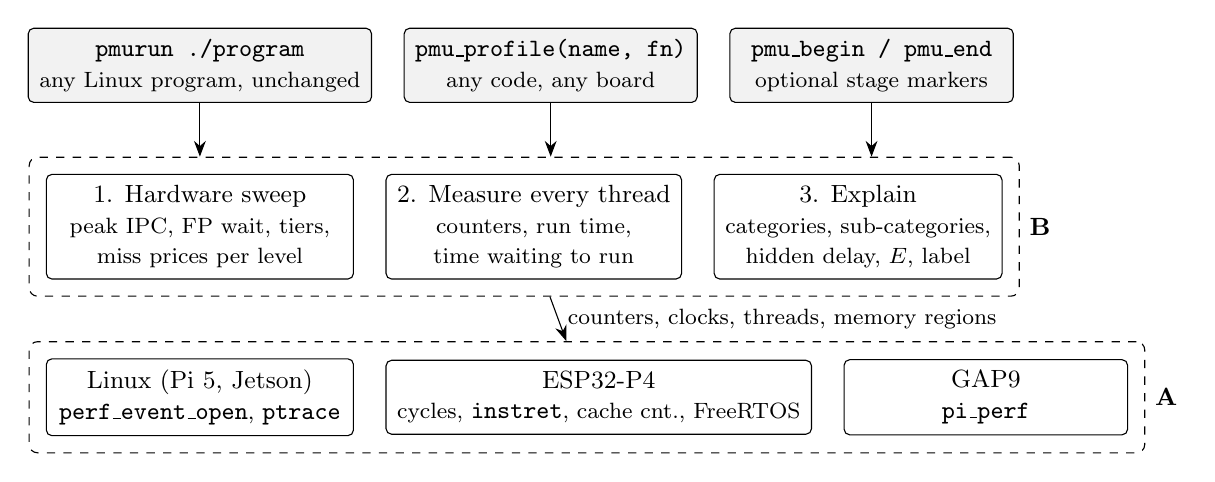
\begin{tikzpicture}[font=\small, box/.style={draw, rounded corners=2pt, align=center, minimum height=8mm, inner sep=4pt},
  part/.style={draw, dashed, rounded corners=3pt, inner sep=6pt}, >={Stealth[length=2mm]}]
\node[box, fill=black!5, minimum width=3.9cm] (e1) {\code{pmurun ./program}\\\footnotesize any Linux program, unchanged};
\node[box, fill=black!5, right=4mm of e1, minimum width=3.6cm] (e2) {\code{pmu\_profile(name, fn)}\\\footnotesize any code, any board};
\node[box, fill=black!5, right=4mm of e2, minimum width=3.6cm] (e3) {\code{pmu\_begin / pmu\_end}\\\footnotesize optional stage markers};
\node[box, below=9mm of e1, minimum width=3.9cm] (sweep) {1. Hardware sweep\\ \footnotesize peak IPC, FP wait, tiers,\\ \footnotesize miss prices per level};
\node[box, right=4mm of sweep, minimum width=3.6cm] (meas) {2. Measure every thread\\ \footnotesize counters, run time,\\ \footnotesize time waiting to run};
\node[box, right=4mm of meas, minimum width=3.6cm] (expl) {3. Explain\\ \footnotesize categories, sub-categories,\\ \footnotesize hidden delay, $E$, label};
\node[part, fit=(sweep)(meas)(expl), label={[font=\small\bfseries]right:B}] (pb) {};
\node[box, below=10mm of sweep, minimum width=3.9cm] (lin) {Linux (Pi 5, Jetson)\\ \footnotesize \code{perf\_event\_open}, \code{ptrace}};
\node[box, right=4mm of lin, minimum width=3.6cm] (esp) {ESP32-P4\\ \footnotesize cycles, \code{instret}, cache cnt., FreeRTOS};
\node[box, right=4mm of esp, minimum width=3.6cm] (gap) {GAP9\\ \footnotesize \code{pi\_perf}};
\node[part, fit=(lin)(esp)(gap), label={[font=\small\bfseries]right:A}] (pa) {};
\draw[->] (e1) -- (e1 |- pb.north); \draw[->] (e2) -- (e2 |- pb.north); \draw[->] (e3) -- (e3 |- pb.north);
\draw[->] (pb) -- node[right, font=\footnotesize]{counters, clocks, threads, memory regions} (pa);
\end{tikzpicture}
\caption{Structure of the harness. Three entry points share Part~B (the method), which is identical on every board; Part~A (the platform layer) is selected at compile time and is the only board-specific code.}
\label{fig:arch}
\end{figure*}

\begin{table}[t]
\centering\footnotesize
\caption{Ways to use the harness.}
\label{tab:use}
\begin{tabularx}{\columnwidth}{|>{\raggedright\arraybackslash}p{2.1cm}|>{\raggedright\arraybackslash}p{1.6cm}|L|}
\hline
\textbf{Entry point} & \textbf{Changes to the program} & \textbf{Measured} \\ \hline
\code{pmurun} (Linux) & none & every thread, from its first instruction to its exit \\ \hline
\code{pmu\_profile} (all) & compiled with the harness & the whole call; each task's share of the core \\ \hline
stage markers (all boards) & marks stages & each stage of each thread \\ \hline
\end{tabularx}
\end{table}

\subsection{Counters and clocks}
The method uses up to thirteen counters, named by \emph{role} rather than by chip-specific event (Table~\ref{tab:counters}). $M_k$ counts accesses that missed in the $k$-th cache level, counted outward from the core; a read that reaches main memory misses at every level and is counted in every $M_k$. The remaining counters describe the instruction mix. Naming by role lets a microcontroller with one cache in front of PSRAM and a board with three cache levels in front of DRAM share one model.

\begin{table}[t]
\centering\footnotesize
\caption{Quantities measured for each thread. All counters are optional.}
\label{tab:counters}
\begin{tabularx}{\columnwidth}{|>{\raggedright\arraybackslash}p{1.6cm}|L|}
\hline
\textbf{Symbol} & \textbf{Meaning} \\ \hline
$C$, $I$ & cycles in the thread's own code; instructions completed \\ \hline
$M_1, M_2, M_3$ & misses at cache levels 1--3 \\ \hline
$S$ & cycles in which the core could not proceed because it was waiting for memory \\ \hline
$LD, ST$ & loads, stores \\ \hline
$INT, FP, SIMD$ & integer, floating-point and SIMD operations \\ \hline
$BR, MISP$ & branches, mispredicted branches \\ \hline
$T_{wall}$ & the thread's lifetime \\ \hline
$T_{run}$ & time the thread was on a core (its code and the kernel working for it) \\ \hline
$T_{delay}$ & time the thread was ready but not running \\ \hline
\end{tabularx}
\end{table}

\subsection{Hardware sweep}\label{sec:sweep}
\code{pmu\_init} opens the counters and runs calibration loops whose behaviour is known exactly. Their results describe the \emph{board} and are then applied to any program.

\paragraph{Peak instruction throughput.} The loop in Listing~\ref{lst:busy} keeps eight independent running sums in registers, touching no memory, so the core retires instructions as fast as its pipeline allows. The empty \code{asm volatile} statement emits no instructions; it prevents the compiler from collapsing or vectorising the loop. The loop runs once unmeasured, so that the clock frequency settles, and once measured, giving $IPC_{peak}=I_{loop}/C_{loop}$ and the length of one cycle, $\tau = T_{cpu}/C_{loop}$.

\begin{lstlisting}[caption={Calibration loop for peak instruction throughput.},label={lst:busy}]
static void busy_loop(long n) {
  /* 8 independent adds: no memory, no dependencies */
  uint32_t a=0, b=0, c=0, d=0, e=0, f=0, g=0, h=0;
  for (long i = 0; i < n; i++) {
    a += i; b += i; c += i; d += i;
    e += i; f += i; g += i; h += i;
    __asm__ volatile("" : "+r"(a), "+r"(b), "+r"(c),
        "+r"(d), "+r"(e), "+r"(f), "+r"(g), "+r"(h));
  }
  sink = a ^ b ^ c ^ d ^ e ^ f ^ g ^ h;
}
\end{lstlisting}

\paragraph{Arithmetic wait.} A single chain of floating-point multiply--adds, in which each operation needs the previous result, gives the extra cycles a dependent floating-point operation waits: $w_{fp} = C_{chain}/FP_{chain} - 1/IPC_{peak}$.

\paragraph{Memory curve.} A buffer of size $s$ is arranged as a single random cycle through its 64-byte lines using Sattolo's algorithm~\cite{sattolo}. Following the chain (Listing~\ref{lst:chase}) visits every line in an order prefetchers cannot predict, and because each load supplies the next address, loads cannot overlap: every step pays the full latency of whichever memory holds the buffer. The chase is repeated for $s = 4\,\mathrm{KB}\times4^k$ in every memory region: one region (up to 64\,MB) on Linux, where caches are found by size; each physical memory separately on microcontrollers (TCM, internal SRAM and PSRAM on the ESP32-P4; L2 on GAP9). Allocations that fail are halved until they succeed.

\begin{lstlisting}[caption={Pointer-chasing loop; each load waits for the previous one.},label={lst:chase}]
static void chase(const uint32_t *p, long n) {
  uint32_t x = 0;
  for (long i = 0; i < n; i++)
    x = p[x * 16];          /* 16 words = 64 B */
  sink = x;
}
\end{lstlisting}

\paragraph{Memory tiers.} A new tier begins wherever the time per access rises by more than a factor of 1.5, or the memory region changes. This uses only the wall clock, so a board without counters still reports its memory structure.

\paragraph{Miss prices.} Across all sweep points, with $N$ accesses each, the cycles per access are fitted by least squares:
\begin{equation}
\frac{C}{N}(s) = c_0 + \sum_{k=1}^{3} p_k\,\frac{M_k}{N}(s).
\end{equation}
Only counters that exist become unknowns; negative prices are set to zero. Because a read that reaches main memory is counted at every level, its cost is $p_1+p_2+p_3$, and each $p_k$ is the extra cost of going one level further. The working sets step through every cache level, so each level's miss rate rises at a different size and the prices are separable.

\paragraph{Counter validation.} A counter that opens but does not work is disabled: an instruction or floating-point counter that barely advances during its loop; a miss counter that never reaches $0.05$ misses per access; a stall counter that records more than $0.2$ stalls per cycle on the add loop, or fewer than $0.5$ on the largest chase.

\subsection{Finding every thread}
In run mode the harness starts the program under \code{ptrace}. The child requests tracing, stops itself and executes the program; the harness asks to be notified of every new thread (\code{PTRACE\_O\_TRACECLONE}), of the program start, and of every thread exit. Linux stops each new thread before its first instruction; the harness then opens that thread's counters and a software task clock, and lets it run. When a thread is about to exit, the harness reads its counters, its running time, its time spent ready but waiting, and its forced and voluntary context-switch counts. Signals sent to the program are forwarded unchanged. Tracing costs a stop per thread creation and exit, not per instruction. On the ESP32-P4, \code{pmu\_profile} reads every FreeRTOS task's running time before and after the call instead.

\subsection{Attribution}\label{sec:attr}
For each thread, the counted work is converted into expected cycles using the measured prices and compared with the measured cycles $C$. The memory part is computed first. The misses multiplied by their prices give the \emph{total} memory latency, as if the misses had occurred one at a time:
\begin{equation}
C_{model} = \sum_{k=1}^{3} p_k M_k .
\end{equation}
The \emph{exposed} memory cycles are bounded by the measured stall cycles, where the board counts them, and by the thread's cycles:
\begin{equation}
C_{mem} = \min\left(C_{model},\; S,\; C\right).
\end{equation}
When misses overlap, $S<C_{model}$ and the measured stalls set the exposed time. When the stall counter includes stalls not caused by memory (the Cortex-A76 provides only a general back-end stall event), $C_{model}$ removes them. $C_{mem}$ is divided among the levels in proportion to $p_kM_k$. The remaining cycles are divided into issuing at full speed, waiting on arithmetic results, and other stalls:
\begin{align}
C_{issue} &= \min\!\left(I/IPC_{peak},\; C - C_{mem}\right), \\
C_{arith} &= \min\!\left(w_{fp}(FP+SIMD),\; C - C_{mem} - C_{issue}\right), \\
C_{stalled} &= C - C_{mem} - C_{issue} - C_{arith}.
\end{align}
Cycles are converted to time with $\tau$. The thread's own code ran for $T_{user}=\tau C$; the rest of its running time was spent by the kernel on its behalf; and the rest of its lifetime it was not running:
\begin{align}
T_{kernel} &= T_{run} - T_{user}, \\
T_{waiting} &= T_{wall} - T_{run} = T_{preempted} + T_{blocked},
\end{align}
with $T_{preempted}=T_{delay}$. Each cycle component is scaled by $T_{user}/T_{wall}$ to become a share of the thread's lifetime.

\paragraph{Categories, sub-categories and labels.} The shares are grouped into five categories that exist on every board, each with sub-categories that appear where the board's counters allow (Table~\ref{tab:cats}). The label is the largest category followed by its largest sub-category, for example \textbf{MEMORY\,/\,L3 misses} or \textbf{WAITING\,/\,preempted}. A board without an L3 cache still has a MEMORY category, so boards can always be compared at the category level, while the sub-categories show the detail each board offers. Without an instruction counter, running time cannot be divided and is labelled \textbf{RUNNING}.

\begin{table}[t]
\centering\footnotesize
\caption{Categories (identical on every board) and sub-categories (where the board can distinguish them).}
\label{tab:cats}
\begin{tabularx}{\columnwidth}{|>{\raggedright\arraybackslash}p{1.45cm}|L|}
\hline
\textbf{Category} & \textbf{Sub-categories} \\ \hline
COMPUTE & issue ($C_{issue}$); waiting on results ($C_{arith}$) \\ \hline
MEMORY & L1, L2, L3 misses (exposed part, by level) \\ \hline
STALLED & other pipeline stalls ($C_{stalled}$) \\ \hline
KERNEL & the operating system working for the thread \\ \hline
WAITING & preempted; blocked (sleep, I/O, locks) \\ \hline
\end{tabularx}
\end{table}

\paragraph{Accuracy and overlap.} The explained fraction $E=(C_{issue}+C_{arith}+C_{mem})/C$ is the share of the measured cycles that the counted work accounts for; the overlap factor $\Omega=C_{model}/C_{mem}$ is close to one when misses occurred one at a time, and greater than one when they overlapped.

\paragraph{Visible and hidden delays.} Shares describe how time was spent; they do not show latency overlapped with useful work. The harness therefore also reports, per thread, the total memory latency $D_{mem}=\tau C_{model}$, its exposed part $D_{exposed}=\tau C_{mem}$, and its hidden part $D_{hidden}=\tau(C_{model}-C_{mem})$, together with the preempted and blocked times. Because many misses can be outstanding at once, $D_{mem}$ may exceed the thread's lifetime. Preempted and blocked time are never hidden: while a thread is not running, it does no work.

\subsection{Output}
For every thread (run mode) or stage (markers), the report contains four tables: (1) \emph{what the code did}: instructions, IPC, loads, stores, integer, floating-point and SIMD operations and branches as a share of instructions, mispredictions as a share of branches, and misses per thousand instructions at each level; (2) the five \emph{categories} as shares of wall time, with the label; (3) the \emph{sub-categories}, with $E$ and $\Omega$; and (4) the \emph{delays}: memory total, exposed and hidden, preempted and blocked time, and forced and voluntary switch counts. Run mode adds a row for the whole program. \code{pmu\_init} has already printed the counters found, the prices and the memory tiers, so every report states what the board could measure.

\subsection{Platform layer}
Table~\ref{tab:platforms} summarises each platform section. On Linux, each counter is opened for one thread, counting user-space events, with the enabled and running times needed to correct for multiplexing. On ARM boards the harness opens an event only if the kernel lists it under \code{/sys/bus/event\_source/devices/armv8*/events/}; the kernel lists only events the core implements, so an L3 event is never opened on a core without L3, and the Cortex-A76 falls back from the memory-specific stall event to the general one.

\begin{table*}[t]
\centering\footnotesize
\caption{Platform layer for the target boards.}
\label{tab:platforms}
\begin{tabularx}{\textwidth}{|>{\raggedright\arraybackslash}p{2.3cm}|L|L|L|}
\hline
\textbf{Item} & \textbf{Linux (Raspberry Pi 5, Jetson Orin Nano)} & \textbf{ESP32-P4 (ESP-IDF)} & \textbf{GAP9 (PMSIS)} \\ \hline
Cycles, instructions & \code{perf\_event\_open}, per thread & \code{esp\_cpu\_get\_cycle\_count}, RISC-V \code{rdinstret} & \code{pi\_perf} \\ \hline
$M_1, M_2, M_3$ & \code{L1D/L2D/L3D\_CACHE\_REFILL} (\code{0x03}, \code{0x17}, \code{0x2A}) & ESP-IDF cache counters: line fills of L1 ($M_1$) and of the L2 PSRAM/flash cache ($M_2$) & not available on the main core \\ \hline
$S$ & \code{STALL\_BACKEND\_MEM} (\code{0x4005}, A78AE); else \code{STALL\_BACKEND} (\code{0x24}, A76) & not needed (in-order) & not needed (in-order) \\ \hline
Instruction mix & \code{LD\_SPEC} \code{0x70}, \code{ST\_SPEC} \code{0x71}, \code{DP\_SPEC} \code{0x73}, \code{VFP\_SPEC} \code{0x75}, \code{ASE\_SPEC} \code{0x74}, \code{BR\_RETIRED} \code{0x21}, \code{BR\_MIS\_PRED\_RETIRED} \code{0x22} & not available & not available \\ \hline
Running time & per-thread CPU clock; software task clock in run mode & FreeRTOS per-task run time & none (single thread) \\ \hline
Preempted vs blocked & \code{/proc/<pid>/task/} \code{<tid>/schedstat} & not separated & not applicable \\ \hline
Finding threads & \code{ptrace} (run mode); \code{/proc/self/task} & \code{uxTaskGetSystemState} & not applicable \\ \hline
Memory regions & RAM, up to 64\,MB & TCM 8\,KB, internal SRAM 256\,KB, PSRAM 4\,MB & L2, 512\,KB \\ \hline
Counter width & 64-bit & 32-bit & 32-bit \\ \hline
\end{tabularx}
\end{table*}

\section{Generalisation to any code and any hardware}

\paragraph{Any code.} The harness never reads, analyses or instruments the program. In run mode it finds every thread itself and attaches counters before the thread's first instruction; the program's thread count, structure and source are irrelevant. Expected time is derived only from work the hardware counted.

\paragraph{Any hardware.} Eight design decisions keep the method valid on unfamiliar boards:
\begin{enumerate}
  \item \textbf{Generic counter roles.} Counters are defined by role, not by event name, so cache-based and scratchpad-based memory systems share one model.
  \item \textbf{Fixed categories, variable detail.} The five categories exist on every board; sub-categories appear only where counters allow, so results remain comparable across boards with different hierarchies.
  \item \textbf{In-order and out-of-order cores.} Measured stall cycles bound the memory time where they exist; on in-order cores the bound is simply absent. Hidden delay is reported either way.
  \item \textbf{Every counter optional and validated.} A counter that is missing or does not behave as expected is disabled; the report contains less detail, never a value from a counter that does not work.
  \item \textbf{Measured prices.} Throughput, arithmetic wait and miss costs come from the board's own sweep, not from datasheets.
  \item \textbf{Memory probed by kind and size.} Caches are found by working-set size; physically separate memories are measured individually.
  \item \textbf{Tiers without counters.} Memory tiers come from timing alone.
  \item \textbf{Robust arithmetic.} 32-bit wrap-around, counter multiplexing and small memories are handled.
\end{enumerate}
Table~\ref{tab:detail} shows the detail available on each target.

\begin{table}[t]
\centering\footnotesize
\caption{Detail available on each target board.}
\label{tab:detail}
\begin{tabularx}{\columnwidth}{|>{\raggedright\arraybackslash}p{1.5cm}|L|L|L|}
\hline
\textbf{Board} & \textbf{Per thread} & \textbf{MEMORY sub-categories} & \textbf{WAITING sub-categories} \\ \hline
Raspberry Pi 5, Jetson Orin Nano & yes, every thread & L1, L2, L3; exposed and hidden & preempted, blocked \\ \hline
ESP32-P4 & task shares of the core$^{\dagger}$ & L1, L2 (PSRAM/flash) & not separated \\ \hline
GAP9 & single thread & none (main core) & not applicable \\ \hline
\multicolumn{4}{|p{0.93\columnwidth}|}{$^{\dagger}$\,Counters are per core; shares from FreeRTOS run-time statistics; to confirm on hardware.} \\ \hline
\end{tabularx}
\end{table}

\section{Validation program}

\subsection{Design principles}
To test the attribution, one needs threads whose correct label is known before they run. The validation program, \code{workload.c}, is an ordinary multi-threaded C program that \emph{contains no harness calls}: the harness must find its threads and explain them exactly as it would for any program. It follows four principles.
\begin{enumerate}
  \item \textbf{One behaviour per thread.} Each thread is built so that a single resource dominates its time, so a wrong label points directly to a flaw in the method.
  \item \textbf{No information given to the harness.} The program does not mark anything; only thread names, which any program may set, identify the rows of the report.
  \item \textbf{Memory threads must leave fast memory.} The buffer is 64\,MB on Linux and 4\,MB of PSRAM on the ESP32-P4, far larger than the caches in front of it.
  \item \textbf{Every category exercised.} The threads together cover COMPUTE, MEMORY with and without hidden latency, WAITING\,/\,blocked and WAITING\,/\,preempted.
\end{enumerate}

\subsection{Threads}
Table~\ref{tab:workload} lists the threads and their expected labels, and Listing~\ref{lst:work} shows their code. The only platform-specific part of the program is how threads are started: POSIX threads on Linux, FreeRTOS tasks on one core of the ESP32-P4, and sequential calls on GAP9, with the amount of work reduced on microcontrollers.

\begin{table*}[t]
\centering\footnotesize
\caption{Threads of the validation program and their expected behaviour.}
\label{tab:workload}
\begin{tabularx}{\textwidth}{|l|L|L|L|>{\raggedright\arraybackslash}p{2.6cm}|}
\hline
\textbf{Thread} & \textbf{What it does} & \textbf{Resource exercised} & \textbf{Expected counter signature} & \textbf{Expected label} \\ \hline
\code{compute} & 4 independent floating-point multiply--add chains in registers & arithmetic units & many FP operations, negligible misses & COMPUTE \\ \hline
\code{rand-mem} & reads the buffer at pseudo-random positions & memory latency & about one miss per read at every level; high hidden share on out-of-order cores & MEMORY / last level \\ \hline
\code{seq-mem} & reads every word of the buffer in order, 8 times & memory bandwidth & about one miss per 64-byte line; latency largely hidden by prefetching & MEMORY (or COMPUTE if fully hidden) \\ \hline
\code{sleeper} & sleeps 2\,ms, then a short loop, 50 times & none (thread blocked) & few instructions; mostly voluntary switches & WAITING / blocked \\ \hline
\code{shared1..3} & the \code{compute} work, all three pinned to one core & the core itself & as \code{compute}; many forced switches & WAITING / preempted ($\approx2/3$) \\ \hline
main & starts the threads and waits for them & none & few instructions & WAITING / blocked \\ \hline
\end{tabularx}
\end{table*}

\begin{lstlisting}[caption={Thread bodies of the validation program (\code{workload.c}); \code{SCALE} reduces work on microcontrollers.},label={lst:work}]
static void compute(void) {
  float a = 1, b = 2, c = 3, d = 4;
  for (long i = 0; i < 40000000L / SCALE; i++) {
    a = a*0.9999f + 1e-4f;  b = b*0.9999f + 1e-4f;
    c = c*0.9999f + 1e-4f;  d = d*0.9999f + 1e-4f;
  }
  sink = (uint64_t)(a + b + c + d);
}
static void rand_mem(void) {
  uint32_t x = 1, s = 0;
  for (long i = 0; i < 8000000L / SCALE; i++) {
    x = x * 1664525u + 1013904223u;     /* LCG */
    s += buf[x % words];
  }
  sink = s;
}
static void seq_mem(void) {
  uint32_t s = 0;
  for (int r = 0; r < 8; r++)
    for (size_t i = 0; i < words; i++) s += buf[i];
  sink = s;
}
static void sleeper(void) {
  for (int r = 0; r < 50; r++) {
    sleep_ms(2);
    uint32_t s = 0;
    for (int i = 0; i < 10000; i++)
      s += (uint32_t)i * r;
    sink = s;
  }
}
\end{lstlisting}

\paragraph{\code{compute}.} Four independent chains let the floating-point unit work in parallel, while each chain waits on its own previous result. The thread tests the instruction-mix counters, the peak-throughput price and the arithmetic-wait price: its label should be COMPUTE, with the sub-category showing whether issue or arithmetic waiting dominates.

\paragraph{\code{rand-mem} and \code{seq-mem}.} Random reads defeat prefetching, so almost every load misses at every level and pays the latency of main memory; consecutive iterations are independent, so on out-of-order cores several misses are in flight and part of the latency is hidden ($\Omega>1$). Sequential reads fetch one line per sixteen loads, and prefetchers fetch ahead, so a large share of their latency should be hidden. Together they test the miss counters, the prices, the stall bound and the hidden-delay measure.

\paragraph{\code{sleeper}, \code{shared1..3} and main.} The sleeper and the main thread spend most of their lives not running by their own choice, and should be labelled WAITING\,/\,blocked with mostly voluntary switches. The three shared threads run the same arithmetic as \code{compute} but are pinned to one core, so the scheduler must divide it among them: each should be WAITING\,/\,preempted about two thirds of the time, with many forced switches, while its running part still shows the COMPUTE signature of \code{compute}. Comparing \code{compute} with \code{shared1} isolates the effect of sharing a core.

A second test, \code{demo.c}, exercises the stage markers, per-thread stage tables and the per-stage list of the threads that used the core.


\section{Preliminary test}\label{sec:prelim}

Before the target boards were available, the run mode was tested on a laptop. The purpose of this test is limited: it exercises the parts of the harness that do not depend on hardware counters, namely finding every thread of an unmodified program, measuring running time, separating preempted from blocked time, and deriving memory tiers from timing. It also checks that the harness degrades as designed when no counters are available.

\begin{table*}[t]
\centering\footnotesize
\caption{Per-thread results of the preliminary test: mean of 3 runs, with the range in brackets. Shares are of each thread's lifetime.}
\label{tab:prelim}
\begin{tabularx}{\textwidth}{|l|c|c|c|c|C|C|l|}
\hline
\textbf{Thread} & \textbf{Lifetime (ms)} & \textbf{Running (\%)} & \textbf{Preempted (\%)} & \textbf{Blocked (\%)} & \textbf{Forced switches} & \textbf{Voluntary switches} & \textbf{Label (all 3 runs)} \\ \hline
main & 165.0 [162.0--170.9] & 3.4 [3.2--3.8] & 4.8 [2.5--6.4] & 91.7 [90.3--93.7] & 3--5 & 18--19 & WAITING / blocked \\ \hline
\code{compute} & 55.7 [54.6--56.5] & 99.2 [98.0--99.9] & 0.0 & 0.8 [0.1--2.0] & 0 & 2 & RUNNING \\ \hline
\code{rand-mem} & 35.7 [33.2--39.5] & 95.2 [88.5--99.6] & 0.0 & 4.8 [0.4--11.5] & 0 & 2 & RUNNING \\ \hline
\code{seq-mem} & 57.6 [57.1--58.2] & 99.1 [98.4--99.7] & 0.0 & 0.9 [0.3--1.6] & 0 & 2 & RUNNING \\ \hline
\code{sleeper} & 120.5 [120.0--121.2] & 0.3 & 0.0 & 99.7 & 0 & 52 & WAITING / blocked \\ \hline
\code{shared1} & 153.2 [148.5--156.8] & 34.2 [33.4--35.2] & 65.3 [64.8--66.1] & 0.5 [0.0--1.5] & 18--27 & 2 & WAITING / preempted \\ \hline
\code{shared2} & 156.3 [155.8--156.7] & 33.4 [33.3--33.5] & 65.1 [64.5--66.0] & 1.6 [0.7--2.1] & 18 & 2 & WAITING / preempted \\ \hline
\code{shared3} & 154.0 [152.9--155.6] & 33.8 [33.4--34.0] & 65.9 [65.3--66.5] & 0.3 [0.0--0.8] & 18--19 & 2 & WAITING / preempted \\ \hline
\end{tabularx}
\end{table*}

\begin{figure*}[t]
\centering
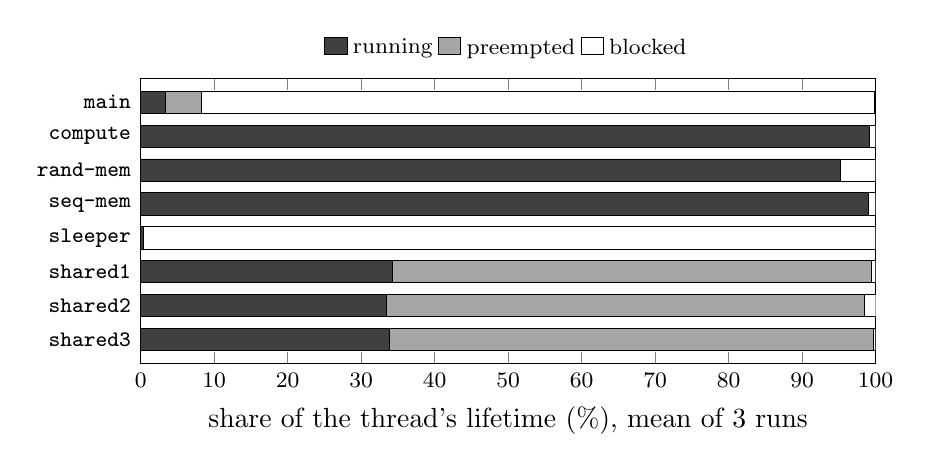
\begin{tikzpicture}
\begin{axis}[xbar stacked, width=0.9\textwidth, height=5.2cm, bar width=8pt, xmin=0, xmax=100,
  xlabel={share of the thread's lifetime (\%), mean of 3 runs}, symbolic y coords={shared3,shared2,shared1,sleeper,seq-mem,rand-mem,compute,main},
  ytick=data, y dir=normal, yticklabel style={font=\footnotesize\ttfamily}, xticklabel style={font=\footnotesize},
  legend style={at={(0.5,1.03)}, anchor=south, legend columns=3, font=\footnotesize, draw=none},
  every axis plot/.append style={draw=black, line width=0.3pt}]
\addplot[fill=black!75] coordinates {(99.2,compute) (95.2,rand-mem) (99.1,seq-mem) (0.3,sleeper) (34.2,shared1) (33.4,shared2) (33.8,shared3) (3.4,main)};
\addplot[fill=black!35] coordinates {(0,compute) (0,rand-mem) (0,seq-mem) (0,sleeper) (65.3,shared1) (65.1,shared2) (65.9,shared3) (4.8,main)};
\addplot[fill=white] coordinates {(0.8,compute) (4.8,rand-mem) (0.9,seq-mem) (99.7,sleeper) (0.5,shared1) (1.6,shared2) (0.3,shared3) (91.7,main)};
\legend{running, preempted, blocked}
\end{axis}
\end{tikzpicture}
\caption{How each thread of the unmodified validation program spent its lifetime in the preliminary test.}
\label{fig:prelim}
\end{figure*}

\subsection{Setup}
Table~\ref{tab:setup} summarises the setup. The laptop is an Apple-silicon MacBook Air. macOS does not give ordinary programs access to the processor's performance counters, and the run mode requires Linux, so the test ran in Linux inside Docker Desktop, which executes containers in a lightweight virtual machine. The virtual machine was given 8 cores. Its hypervisor does not expose the performance monitoring unit, so no hardware counter is available; this is the case the harness must handle without producing incorrect values. The harness and the validation program were compiled inside the container and the program was profiled three times (Listing~\ref{lst:cmd}). The thread bodies are those of Listing~\ref{lst:work}; Listing~\ref{lst:start} shows how the program starts its threads, including the pinning of the three shared threads to one core. Neither listing contains any call to the harness.

\begin{table}[t]
\centering\footnotesize
\caption{Setup of the preliminary test.}
\label{tab:setup}
\begin{tabularx}{\columnwidth}{|>{\raggedright\arraybackslash}p{2.0cm}|L|}
\hline
\textbf{Item} & \textbf{Value} \\ \hline
Host & Apple-silicon MacBook Air, macOS \\ \hline
Linux environment & Docker Desktop 29.9 (Linux virtual machine), image \code{gcc:14} \\ \hline
Cores available & 8 \\ \hline
Hardware counters & none exposed (\code{counters: none}) \\ \hline
Scheduler statistics & available (\code{schedstat}): preempted and blocked time separated \\ \hline
Program & \code{workload.c}, unmodified, 8 threads \\ \hline
Runs & 3 \\ \hline
\end{tabularx}
\end{table}

\begin{lstlisting}[language=bash,caption={Commands used for the test (run in the folder containing the source).},label={lst:cmd}]
docker run --rm --privileged -v "$PWD":/h -w /h gcc:14 \
  bash -c "gcc -O2 pmu.c pmurun.c -o pmurun -pthread &&
           gcc -O2 workload.c -o workload -pthread &&
           nproc &&
           for i in 1 2 3; do ./pmurun ./workload; done" \
  | tee mac_docker.txt
\end{lstlisting}

\begin{lstlisting}[caption={How the validation program starts its threads on Linux (\code{workload.c}); no harness call is involved.},label={lst:start}]
static void *run_job(void *a) {
  job_t *j = a;
  pthread_setname_np(pthread_self(), j->name);
  if (j->pin >= 0) {          /* shared1..3: one core */
    cpu_set_t one; CPU_ZERO(&one); CPU_SET(j->pin, &one);
    pthread_setaffinity_np(pthread_self(),
                           sizeof one, &one);
  }
  j->fn();
  return NULL;
}
static void run_all(job_t *jobs, int n) {
  pthread_t th[16];
  for (int i = 0; i < n; i++)
    pthread_create(&th[i], NULL, run_job, &jobs[i]);
  for (int i = 0; i < n; i++)
    pthread_join(th[i], NULL);
}
\end{lstlisting}

\subsection{Results}

\paragraph{Board profile.} In all three runs the harness reported that no counters were available and therefore that only running and waiting could be distinguished. The memory sweep, which needs only the wall clock, found four tiers (Table~\ref{tab:tiers}).

\begin{table}[t]
\centering\footnotesize
\caption{Memory tiers found by the sweep (time per dependent access, mean of 3 runs).}
\label{tab:tiers}
\begin{tabularx}{\columnwidth}{|c|>{\raggedright\arraybackslash}p{2.2cm}|c|L|}
\hline
\textbf{Tier} & \textbf{Working sets} & \textbf{ns / access} & \textbf{Consistent with} \\ \hline
T0 & 4--64 KB & 1.9 & private L1 data cache \\ \hline
T1 & 256 KB--4 MB & 6.2--7.7 & shared L2 cache \\ \hline
T2 & 16 MB & 26.4 & beyond L2: system-level cache and DRAM \\ \hline
T3 & 64 MB & 94.8 & DRAM \\ \hline
\end{tabularx}
\end{table}

\paragraph{Threads.} All eight threads were found in every run, named as the program named them, from their first instruction to their exit. Table~\ref{tab:prelim} gives the mean over the three runs with the range, and Figure~\ref{fig:prelim} shows how each thread's lifetime divides. Without counters the running part cannot be divided further and is reported as RUNNING, as specified in Section~\ref{sec:attr}.





\subsection{Analysis}

\paragraph{Finding threads.} The harness found every thread of a program that contains no harness code, in every run, which is the central requirement of run mode (R1). The thread count did not need to be known in advance.

\paragraph{Preemption.} The three shared threads, pinned to one core, each ran $33.4$--$34.2\%$ of their lifetime and were preempted $65.1$--$65.9\%$ of it, with 18 to 27 forced switches each: the scheduler divided the core almost exactly into thirds, and the harness attributed the remaining two thirds to WAITING\,/\,preempted. The result is internally consistent: each shared thread ran for about $0.34\times154\approx52$\,ms, close to the $55.7$\,ms the identical \code{compute} thread needed on its own core, and their lifetime of about $154$\,ms is close to three times that work. The extra time is therefore correctly explained as waiting for the core, not as slower execution.

\paragraph{Blocking.} The sleeper was blocked $99.7\%$ of its lifetime, with 52 voluntary switches (its 50 sleeps plus thread start and exit), and the main thread, which only waits for the others, was blocked $90$--$94\%$. Both received the expected label. The measured blocked time of the sleeper, $120.1$\,ms for fifty requested sleeps of 2\,ms, shows that each sleep lasted about $2.4$\,ms: the harness quantifies the operating system's sleep overshoot, a property of the platform rather than of the program. The main thread was also preempted for $2.5$--$6.4\%$ of its life, while the seven worker threads competed for the cores.

\paragraph{Independent threads.} \code{compute}, \code{rand-mem} and \code{seq-mem} each had a core of their own and ran $95$--$99\%$ of their lifetimes, with no preemption. Without counters, their running time cannot be divided into COMPUTE, MEMORY and STALLED, and the harness labelled them RUNNING, as designed. This is the expected limitation of a virtual machine without counters, not an error: the harness stated at start-up that no counters were found and printed a dash for every quantity it could not measure.

\paragraph{Memory tiers.} The sweep recovered four tiers from timing alone (Table~\ref{tab:tiers}), with a $1.9$\,ns first level, a second level of $6$--$8$\,ns up to 4\,MB, a transition at 16\,MB, and DRAM at about $95$\,ns. These values are consistent with a private L1 cache, a shared L2 cache, a system-level cache and DRAM. They show that the tier detection works even when the board, here a virtual machine, exposes no counters.

\paragraph{Repeatability.} Lifetimes and shares varied by a few percent between runs, with one exception: in the third run, \code{rand-mem} was blocked for $11.5\%$ of its lifetime instead of $0.4$--$2.6\%$. The cause was not identified; an interruption by the host system of the virtual machine is the most likely explanation. The harness classified the interval as time not running rather than as slower execution, and the episode illustrates why results should be reported over repeated runs.

\paragraph{Summary.} The test confirms, on an unmodified program, the thread discovery of run mode, the separation of running, preempted and blocked time, the expected WAITING labels and sub-categories, the timing-only memory tiers, and the explicit handling of missing counters. The counter-based parts of the method---the instruction mix, the COMPUTE, MEMORY, STALLED and KERNEL categories, and the visible and hidden memory delays---require a board that exposes its counters, and are the subject of the evaluation on the target boards.

\section{Evaluation plan}
Following the preliminary test, the harness will be evaluated on each target board by running the validation program unchanged, now with hardware counters. For each board we will report:
\begin{itemize}
  \item \textbf{Board profile:} counters found, $IPC_{peak}$, $w_{fp}$, the prices $p_k$, and the memory tiers;
  \item \textbf{Label correctness:} whether each thread receives its expected label and sub-category;
  \item \textbf{Accuracy:} $E$ and $\Omega$ per thread, and the hidden share of memory latency;
  \item \textbf{Scheduling:} whether the shared threads are preempted about two thirds of the time, and the sleeper and main thread are blocked;
  \item \textbf{Repeatability:} the variation of shares across repeated runs;
  \item \textbf{Overhead:} the program's run time with and without the harness.
\end{itemize}
Comparing the category tables across boards tests the central claim: that one unchanged program, profiled by one unchanged harness, yields correct and comparable explanations on very different hardware.

\section{Limitations}
\begin{itemize}
  \item \textbf{Counter multiplexing.} With more events than counters, counts are estimated from the fraction of time each was active; very short threads may have imprecise counts.
  \item \textbf{General stall event on the Cortex-A76.} The bound $\min(C_{model},S)$ removes stalls with no counted misses, but a thread that mixes misses with long-latency arithmetic may attribute some arithmetic stalls to memory.
  \item \textbf{Arithmetic wait is an upper bound per operation.} $w_{fp}$ is measured for fully dependent operations; it is capped by the cycles left, and only floating-point and SIMD operations are priced. Integer division and other long-latency operations remain in STALLED.
  \item \textbf{Clock frequency.} $\tau$ is measured once; boards should run with a fixed (performance) frequency governor while measuring.
  \item \textbf{Caches the core cannot see.} A system-level cache outside the CPU cluster, such as the Jetson Orin Nano's, is not counted by core events; its hits appear as main-memory accesses with a lower average price.
  \item \textbf{Microcontrollers.} On the ESP32-P4 the counters are per core, so a profile covers everything the core ran; each task's share comes from FreeRTOS, and waiting is not split into preempted and blocked. GAP9's main core runs one thread and has no memory events. The ESP32-P4 instruction counter and task statistics, and the GAP9 build files, remain to be confirmed on hardware.
\end{itemize}

\section{Conclusion}
We presented a small, portable harness that profiles how a board runs any program. It separates what is known about the \emph{board}, obtained once by a hardware sweep, from what is counted about each \emph{thread} while the program runs, and compares the expected time of the counted work with the measured time. On Linux boards it requires no change to the program and finds every thread itself. Its five categories are the same on every board, its sub-categories expose the detail each board offers, and it distinguishes visible from hidden delays and preempted from blocked time. A preliminary test on a laptop, without counters, confirmed the thread discovery, the scheduling categories and the timing-only memory tiers. The next steps are to run the validation program on the four target boards, to extend the GAP9 port to the cluster cores, and to profile real applications across the boards.

\begin{thebibliography}{9}\small
\bibitem{lmbench} L.~McVoy and C.~Staelin, ``lmbench: Portable tools for performance analysis,'' in \emph{Proc. USENIX Annual Technical Conference}, 1996.
\bibitem{perfman} Linux man-pages project, ``\code{perf\_event\_open}(2) --- set up performance monitoring.''
\bibitem{papi} P.~J.~Mucci, S.~Browne, C.~Deane, and G.~Ho, ``PAPI: A portable interface to hardware performance counters,'' in \emph{Proc. Department of Defense HPCMP Users Group Conference}, 1999.
\bibitem{roofline} S.~Williams, A.~Waterman, and D.~Patterson, ``Roofline: An insightful visual performance model for multicore architectures,'' \emph{Communications of the ACM}, vol.~52, no.~4, pp.~65--76, 2009.
\bibitem{topdown} A.~Yasin, ``A Top-Down method for performance analysis and counters architecture,'' in \emph{Proc. IEEE International Symposium on Performance Analysis of Systems and Software (ISPASS)}, 2014.
\bibitem{sattolo} S.~Sattolo, ``An algorithm to generate a random cyclic permutation,'' \emph{Information Processing Letters}, vol.~22, no.~6, pp.~315--317, 1986.
\bibitem{espidf} Espressif Systems, \emph{ESP-IDF Programming Guide}, ESP32-P4.
\bibitem{gapsdk} GreenWaves Technologies, \emph{GAP SDK and PMSIS API documentation}.
\end{thebibliography}

\end{document}
